\documentclass{article}
\usepackage[utf8]{inputenc}
\usepackage{graphicx}

\title{PS6}
\author{Kevin McGuire}
\date{March 3, 2020}

\begin{document}

\maketitle

\section{Data Description}
The data I used for this project is an example of what I will use for my final project. The data goes through a number of steps as it is transformed from the raw tweets from each candidate to a usable output. The scripts for each step can be found under the TwitterProject folder. The tweets are first cleaned with Clean Tweets.R, extracting only the text, and then generating a sentiment score for each tweet. These tweet/sentiment files are saved in this format for each day. In the next step, Consolidate Sentiment.R these individual sentiment files are combined into one file for each candidate for the desired date range. These combined files are then summarized by Generate Statistics.R, which will provide a variety of measures of daily volume and sentiment for each candidate. The output from this step can then be used in Generate Graphics.R to create visualizations.
\newline
\newline
Generate Graphics.R can also create visualizations of polling averages as calculated by FiveThirtyEight, which are collected and parsed by Get Polling Average.R.

\section{Visualizations}
\begin{figure}[h!]
    \centering
    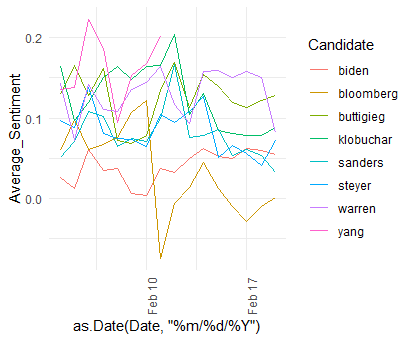
\includegraphics[width=.4\linewidth]{Average_Sentiment.png}
    \caption{Average Sentiment}
\end{figure}

This graphic presents the average sentiment from each tweet tagging each candidate by day. It shows whether a candidate is getting generally positive or negative responses on Twitter, though it does not distinguish between a polarizing candidate and a generally boring one.

\begin{figure}[h!]
    \centering
    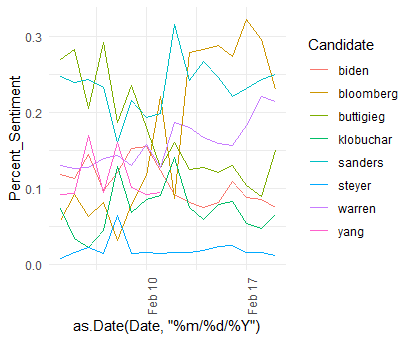
\includegraphics[width=.4\linewidth]{Percent_Sentiment.png}
    \caption{Percent Sentiment}
\end{figure}

This graphic presents the how much of the total primary sentiment (in absolute terms) are directed towards each candidate by day. This shows when candidates have polarizaing moments.

\begin{figure}[h!]
    \centering
    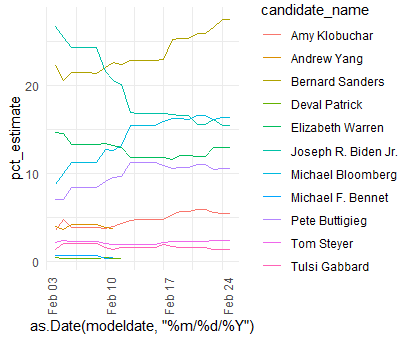
\includegraphics[width=.4\linewidth]{Polling_Average.png}
    \caption{Average Sentiment}
\end{figure}

This graphic shows the polling average for each candidate over time. It will serve as one form of comparison for my model's accuracy.

\end{document}
